\section{Ethereum}
\subsection{ERC-20}
Token contract keeps track of fungible tokens.
Can be used as vault for NFTs.
The ERC-20 token standard supported the implementation of a standard API or Application Programming Interface for tokens in smart contracts. 
So, ERC20 serves as a standard protocol for the Ethereum blockchain and enables users to share, exchanging or transfer tokens.

\subsubsection{Code Functions}
\paragraph{Mandatory}
\begin{lstlisting}
  #How many tokens are in circulation. (read)
  function totalSupply() public view returns (uint256)

  #How many tokens has the address. (read)
  function balanceOf(address _owner) public view returns (uint256 balance)

  function transfer(address _to, uint256 _value) public returns (bool success)
  function transferFrom(address _from, address _to, uint256 _value) public returns (bool success)
  function approve(address _spender, uint256 _value) public returns (bool success)
  function allowance(address _owner, address _spender) 9public view returns (uint256 remaining)
\end{lstlisting}
\paragraph{Optional (But recommended)}
\begin{lstlisting}
  function name() public view returns (string)
  function symbol() public view returns (string)
  function decimals() public view returns (uint8)
\end{lstlisting}
\paragraph{Events}
\begin{lstlisting}
  #Triggered by transfer. Smart Contract cannot react to Event. Client outside of contract needed.
  event Transfer(address indexed _from, address indexed _to,uint256 _value)
  
  #Needed if you want to give someone else permission to transfer.
  event Approval(address indexed _owner, address indexed _spender, uint256 _value)
\end{lstlisting}

\paragraph{Statements}
\begin{lstlisting}
  #Is used to check for code that should never be false. Failing assertion probably means that there is a bug. Uses up all the remaining gas and reverts all the changes made.
  assert()

  #is used to validate inputs and conditions before execution. Reverts back all the changes made to the contract but does refund all the remaining gas fees we offered to pay. 
  require()

  #is used abort execution and revert state changes
  revert()
\end{lstlisting}

\subsubsection{Implementation}
OpenZeppelin - many default contracts, very good source.

\subsubsection{Dividends}
Loop over accounts does not work. 
TotalDrop always increasing.
Every account knows if bonus payed out.
Call updateAccount() on every transfer.
User claims bonus.

\begin{lstlisting}
  function claimBonus() public payable {
    Account storage account = updateAccount(msg.sender);
    uint256 sendValue = account.bonusWei;
    account.bonusWei = 0;
    msg.sender.transfer(sendValue);
  }
  uint256 public totalDrop = 0;
  uint256 public rounding = 0;
  struct Account {
    uint256 lastAirdropWei;
    uint256 bonusWei;
    uint256 valueToken;
  }
  mapping(address => Account) public accounts;

  function() public payable {
    uint256 value = msg.value + rounding;
    rounding = value % totalSupply;
    uint256 weiPerToken = (value - rounding) / totalSupply;
    totalDrop += weiPerToken;
  }

  function updateAccount(address _addr) internal {
    Account storage account = accounts[_addr];
    uint256 weiPerToken = totalDrop - account.lastAirdropWei;
    if(weiPerToken != 0) {
      account.bonusWei += weiPerToken * account.valueToken;
      account.lastAirdropWei = totalDrop;
    }
  }
\end{lstlisting}

\subsubsection{Considerations}

\subsection{Random Numbers}
There is no random number in Ethereum, because every EVM (Node) needs to come to the same result.

\subsubsection{Alternative}
\begin{enumerate}
  \item Random Numbers from Oracle (External source)
  \item Commitment schemes
\end{enumerate}
 
\paragraph{Commitment Scheme - Conflip}
\begin{enumerate}
  \item Alice flips coin, adds it to a random number
  \begin{itemize}
    \item e.g.: tail\#randomnumber1234
    \item hashes it
    \item commitment = sha256(tail\#randomnumber1234)
  \end{itemize}
  \item Alice sends the commitment to Bob and tells bob to flip the coin.
  \item Bob flips coin and sends head to Alice.
  \item Alice reveals the random number, Bob can verify that the commitment was tail.
  \item Both same, Alice wins, both different, Bob wins.
  \item Alice: tail, Bob: head $\rightarrow$ Bob wins.
\end{enumerate}
Step 4) here you can try to cheat! 
Alice knows the result before Bob, so she can just not send the number to Bob.
Therefore, add a amount to the commitment, so Alice pays before the commitment and loses the amount if she does not send the number.

\paragraph{Blockhash}
Only up to 256 blockhashes from the past can be accessed.
Deduct / add tokens / ETH from the past address.
Miner can influence the random value in a sense.

\begin{lstlisting}
  function transfer(address _to, uint256 _value) public returns (bool) {
    //since this is a lucky coin, the value transferred is not what you expect
    luckyTransfer();
    previousTransferBlockNr = block.number;
    previousTransferAddress = msg.sender;

    uint256 val -= potIncrease;
    pot += potIncrease;
  }
  function luckyTransfer() private {
    if(block.number != previousTransferBlockNr && (block.number - previousTransferBlockNr) < 256 ) {
      uint256 rnd = uint256(
        keccak256(
          block.blockhash(previousTransferBlockNr)
        )
      );
      if(rnd % 200 == 0) { //.5%
        balances[previousTransferAddress] += pot;
        Emit Transfer(this, previousTransferAddress, pot);
        //tokens are from pot, thus no tokens are created from thin air
        pot = 0;
        previousTransferBlockNr = 0;
        previousTransferAddress = 0;
      }
    }
  }
\end{lstlisting}




\subsection{ERC-721}
There is either one NFT or there are none.
The standards in ERC-721 tokens focus on critical aspects for deciding ownership and approaches for the creation of tokens.
The standards also dictate the approaches for destroying and transferring the tokens. 


\paragraph{Pros}
\begin{itemize}
  \item Trade items without middleman
  \item Works 24/7
  \item Only digital
\end{itemize}
\paragraph{Cons}
\begin{itemize}
  \item Technical complexity
  \item NFTs on Ethereum not environment friendly
  \item Only digital
  \item Owning tokens does not necessarily mean owning copyright (unless it is explicitly transferred)
\end{itemize}

\subsubsection{Implementation}
\begin{lstlisting}
  #Balance of NFTs of an owner
  function balanceOf(address _owner) external view returns (uint256);

  #Queries the owner of a specific NFT
  function ownerOf(uint256 _tokenId) external view returns (address);

  #Transfer token of owner, or of approved owner in a safe manner (calls onERC721Received)
  function safeTransferFrom(address _from, address _to, uint256 _tokenId, bytes data) external payable;
  function safeTransferFrom(address _from, address _to, uint256 _tokenId) external payable;

  #Make sure you have the right address
  function transferFrom(address _from, address _to, uint256 _tokenId) external payable;

  #Set approve that other address can transfer NFTs
  function approve(address _approved, uint256 _tokenId) external payable;
  function setApprovalForAll(address _operator, bool _approved) external;

  #Check approval
  function getApproved(uint256 _tokenId) external view returns (address);
  function isApprovedForAll(address _owner, address _operator) external view returns (bool);

  #ERC165 - mandatory! XOR of all function signatures
  function supportsInterface(bytes4 interfaceId) external view returns (bool);
  return interfaceId == type(IERC721).interfaceId || interfaceId == type(IERC721Metadata).interfaceId || interfaceId == type(IERC165).interfaceId;
\end{lstlisting}

\paragraph{Events}
\begin{lstlisting}
  event Transfer(address indexed _from, address indexed _to, uint256 indexed _tokenId);
  event Approval(address indexed _owner, address indexed _approved, uint256 indexed _tokenId);
  event ApprovalForAll(address indexed _owner, address indexed _operator, bool _approved);
\end{lstlisting}
\paragraph{Metadata}
\begin{lstlisting}
  function name() external view returns (string _name);
  function symbol() external view returns (string _symbol);
  function tokenURI(uint256 _tokenId) external view returns (string);
\end{lstlisting}

\paragraph{Optional}
Make NFT discoverable
\begin{lstlisting}
  function totalSupply() external view returns (uint256);
  function tokenByIndex(uint256 _index) external view returns (uint256);
  function tokenOfOwnerByIndex(address _owner, uint256 _index) external view returns (uint256);
\end{lstlisting}

\paragraph{Imports}
\begin{lstlisting}
  #import interface instead of all functions
  // SPDX-License-Identifier: MIT
  pragma solidity ^0.8.9;
  import "@openzeppelin/IERC721.sol";
  import "@openzeppelin/IERC721Metadata.sol";

  contract BlChNFT is IERC721 {
    
  }
\end{lstlisting}

\section {ERC20 vs. ERC721}

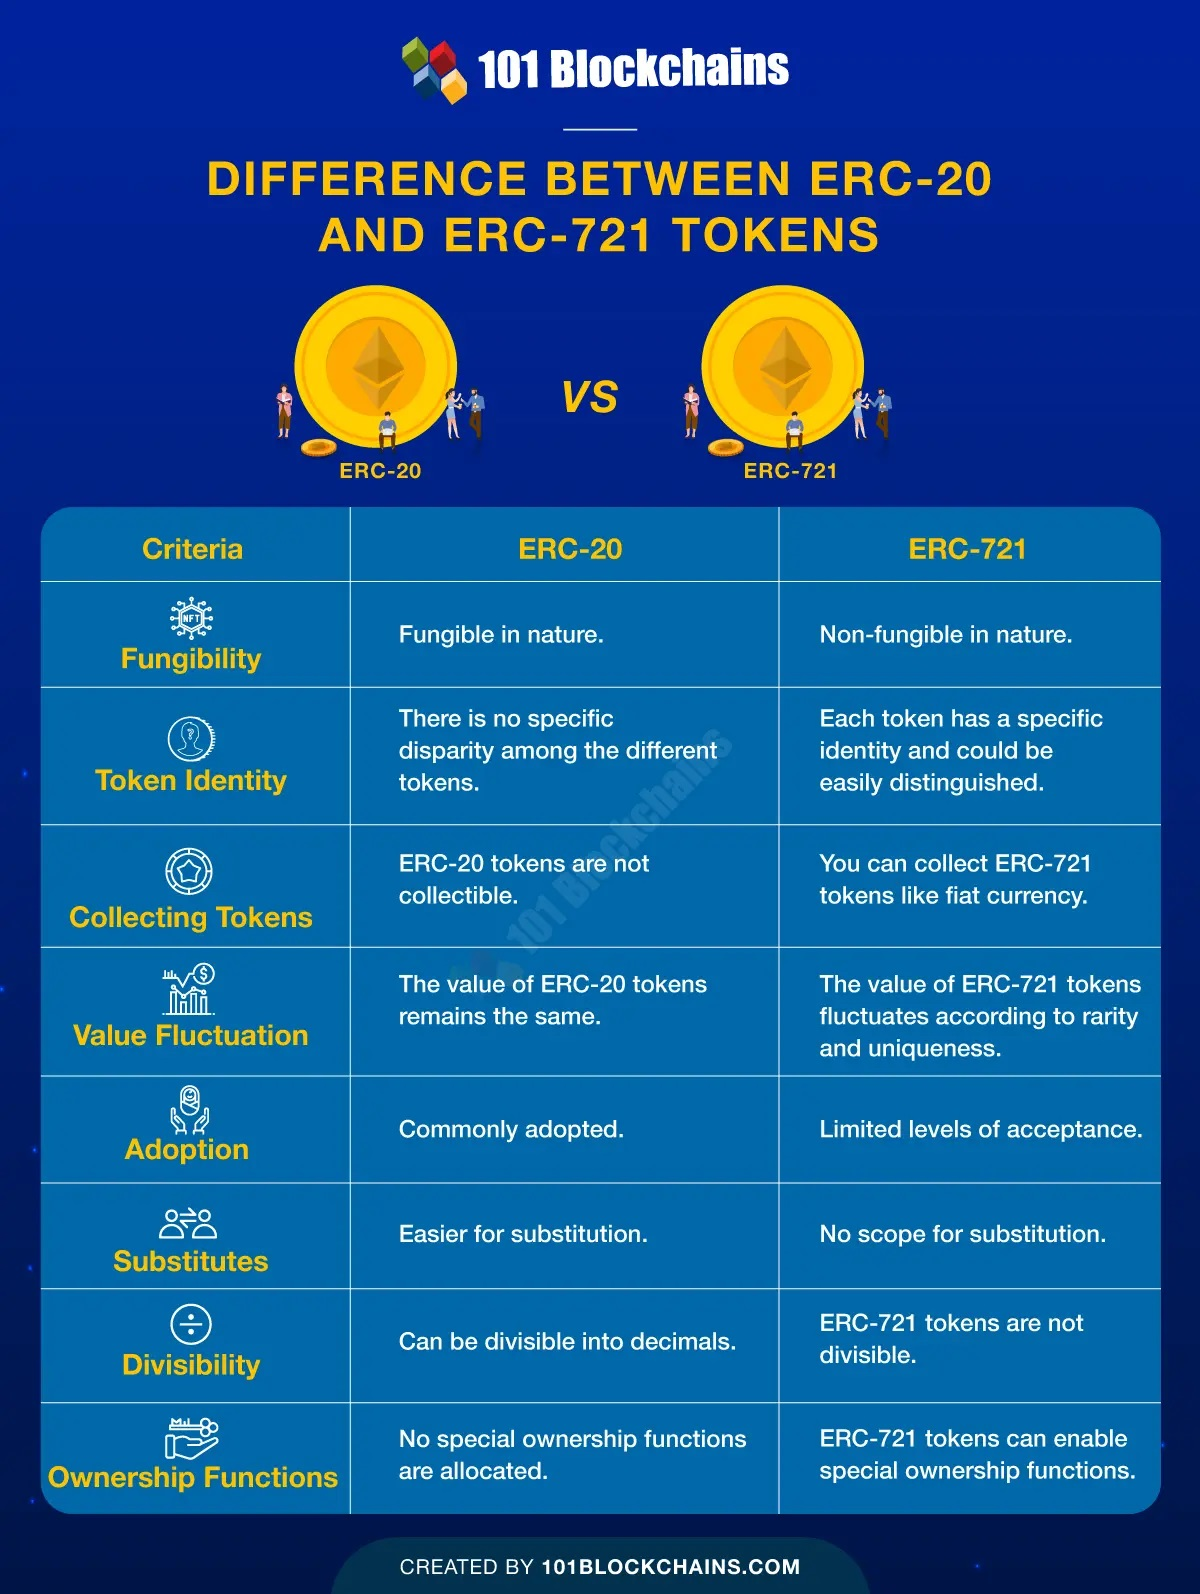
\includegraphics[width=\linewidth]{erc-difference.jpg}